\documentclass[output=paper]{langsci/langscibook}

\author{Julie Fadlon\affiliation{Tel Aviv University}\and
        Julia Horvath\affiliation{Tel Aviv University}\and
        Tal Siloni\affiliation{Tel Aviv University}\lastand
        Ken Wexler\affiliation{Massachusetts Institute of Technology}}

\title{The verbal passive: No unique phrasal idioms}

% \chapterDOI{} %will be filled in at production

\abstract{The paper reports and discusses two studies we conducted to
    systematically assess the distribution of \ili{English} phrasal \isi{idioms} across
    various diatheses (transitive, unaccusatives, adjectival and verbal
    passives). Both studies, a quantitative survey of idiom dictionaries and an
    experiment using invented \isi{idioms}, show that the distribution of
    phrasal \isi{idioms} depends on the diathesis of the idiom’s head. While
    transitives, unaccusatives and adjectival passives can head \isi{idioms} specific
    to them, verbal passive\is{passive} \isi{idioms} uniformly have a transitive (active)
    version. This pattern, we argue, shows that phrasal \isi{idioms} are stored in
    the (pre-syntactic) lexicon as subentries of the entry of their head (not
    as independent entries). Further, it reinforces proposals that the verbal
    passive\is{passive} is a post-lexical output, which consequently lacks its own lexical
    entry, contrasting in this respect with the other diatheses we examined.
    Our findings also provide evidence that the lexicon comprises derived
    entries, which we take as indication that it is an active component of
    grammar.}

\maketitle

\begin{document}\glsresetall

\section{Introduction}

It has sporadically been observed in the literature that there is a gap in the
distribution of \isi{idioms}. Specifically, \citet{DubSim1996}, \citet{Marantz1997},
and \textcite{Ruwet1991} report that in \ili{Chichewa}, \ili{English}, and
\ili{French} there do not seem to be any \isi{idioms} specific to
the verbal (eventive) passive\is{passive} (e.g., \emph{sold} as in \textit{the first costumer was
sold the car}), while there are \isi{idioms} specific to the adjectival (stative)
passive (e.g., \emph{shaven}). In other words, an idiom\is{idioms} in the verbal passive
must have a transitive (active) version.

A first quantitative survey checking the validity of these observations is
reported in \citet{HorSil2009} regarding \ili{Hebrew}. The survey examined four
diatheses: the verbal passive\is{passive}, adjectival passive\is{passive}, transitive, and
unaccusative. The results of the survey showed that the unaccusative\is{unaccusativity} and
adjectival passive\is{passive} diatheses can have \isi{idioms} that do not have a transitive
version, and \isi{idioms} in the transitive diathesis do not necessarily have an
unaccusative version, as illustrated in (\ref{ex:20.1}--\ref{ex:20.3}) below. But the verbal passive
always shares its idiomatic meaning with the transitive alternant (``\#'' means the
corresponding sequence of words does not have an idiomatic
meaning.)\footnote{The citation form in \ili{Hebrew} is third person singular
    past; glosses and translations match this; the \isi{idioms}, of course, are not
    limited to the past tense. For the sake of clarity, a lexically non-fixed
    constituent in \ili{Hebrew} \isi{idioms} is marked by \emph{x}.}\largerpage[2]

\ea\label{ex:20.1} \ili{Hebrew}
    \ea Unaccusative\\
       \gll    yaca  le-\emph{x} me-ha-af \\
                went.out to-\emph{x} from-the-nose \\
            \glt    \enquote*{got tired of}
    \ex Transitive\\
    \gll \# hoci   le-\emph{x} me-ha-af \\
        {} took.out to-\emph{x} from-the-nose \\
    \z
\ex \label{ex:20.2} \ili{Hebrew}
    \ea Adjectival passive\\
        \gll    dafuk   ba-roš \\
                knocked in.the-head \\
            \glt    \enquote*{stupid}
    \ex Transitive\\
    \gll  \# dafak et \emph{x} ba-roš \\
          {} knocked \Acc{} \emph{x} in.the-head \\
    \z
\ex \label{ex:20.3} \ili{Hebrew}
    \ea Transitive\\
         \gll    hosif šemen la-medura \\
                added oil to.the-fire \\
        \glt   \enquote*{worsened a difficult situation via a certain act},
    \enquote*{added fuel to the fire}
    \ex Unaccusative\\
        \gll  \#  nosaf šemen la-medura\\
              {}  got.added oil  to.the-fire \\
    \z
\z

Further, \textcite{SilHorKluWex2018} report an experiment on \ili{Hebrew}
speakers that reinforces the claim that the distribution of phrasal idioms
depends on the diathesis of their head. Participants in the experiment
perceived the likelihood of the verbal passive\is{passive} to share idiomatic meanings with
its transitive counterpart as significantly higher than that of both the
adjectival passive\is{passive} and the unaccusative\is{unaccusativity}.

This paper advances the claim that the reason why the verbal passive\is{passive} differs
from the other diatheses regarding the ability to appear in \isi{idioms} specific to
the diathesis is an inherent (independently motivated) difference between the
former and the latter that affects the storage possibilities available to each.

As is well known, \isi{idioms} exhibit an inherent duality. On the one hand, they are
associated with an unpredictable, conventionalized meaning, which must be
stored (listed) in mental representations. On the other hand, they are units
with internal syntactic structure parallel to units built in the syntax.
Further, \isi{idioms} are constructs that interact with grammar – they can be
embedded, can allow passivization, etc. This means that they must be stored
intra-grammatically, that is, in the lexical component of grammar. We will
claim that \isi{idioms} in the verbal passive\is{passive} cannot be stored the way the adjectival
passive, unaccusative\is{unaccusativity} (more generally, anticausative) and transitive \isi{idioms} are
stored. This, in turn, will account for their inability to head their \enquote{own}
idioms.

The paper first addresses the question of the crosslinguistic validity of the
quantitative results mentioned above with regard to \ili{Hebrew}. This is
particularly important since the verbal passive\is{passive} in \ili{Hebrew} is known to
occur with relatively low frequency in spoken language in comparison to its
English counterpart \citep{Berman2008}. This may be argued to potentially
affect the inventory of verbal passive\is{passive} \isi{idioms} in \ili{Hebrew}. It is thus
essential to examine the situation in another language, where usage of the
verbal passive\is{passive} is more frequent. In order to do that, we conducted a
quantitative study of the distribution of \isi{idioms} in \ili{English}.

Two additional factors make this comparative extension even more worthwhile.
First, the passive\is{passive} morphology in \ili{Hebrew} versus \ili{English} is of a different
type.  While the \ili{Hebrew} verbal passive\is{passive} is formed by means of a verbal
template, in \ili{English}, the verbal passive\is{passive} is periphrastic, and formed by use of
an auxiliary\is{auxiliaries} verb. Second, a comparative study by \citet{Meltzer-Asscher2012}
argues that the verbal passive\is{passive} in \ili{English} versus \ili{Hebrew} also differ with
regard to the realization of the demoted external θ-role. While in \ili{English}
various diagnostics detect the syntactic presence of the external θ-role
\parencite[e.g.][]{Jaeggli1986,BakJohRob1989,Collins2005}, in \ili{Hebrew}, the
role is not syntactically present, but is assigned to a variable in the
semantic representation (along lines suggested by
\citealt{Chierchia2004,Reinhart2002,HorSil2009}, among others).

Since the term ``idiom'' is pre-theoretic and refers to various types of fixed
expressions, we adopted \citeauthor{HorSil2017}’s
(\citeyear{HorSil2017,HorSil2019}) definition identifying a core set of
\isi{idioms}, which has allowed us to test a coherent set of expressions. The
set consists of conventionalized multilexemic expressions whose meaning is
figurative (metaphoric) and unpredictable by semantic composition.\footnote{For
    the sake of clarity, it is worth noting that a property often mistakenly
    conflated with the unpredictability of idioms’ meaning is the level of
    opacity or transparency of their meaning. Idioms indeed differ from one
    another in the level of their transparency (opacity).  For example, the
    idiom\is{idioms} in (ii) may be felt less transparent than the one in (i).  However,
    the degree of transparency can be determined only once we know the meaning
    of the idioms; neither the former nor the latter meanings can be predicted
    based on the meaning of their building blocks. Hence, the meanings of (i)
    is unpredictable (even if a posteriori, more transparent) just like that of
    (ii). Both types of \isi{idioms} are included in our study.

    \ea     land on one’s feet\\
            \glt ‘make a quick recovery’
        \ex cool one’s heels\\
            \glt \enquote*{wait}
    \z}

Further, following \textcite{HorSil2017,HorSil2019}, we distinguish between\linebreak
phrasal and clausal idioms: the former are headed by a lexical head, while the
latter involve sentential functional material such as tense etc., as defined in
\REF{ex:20.4}, and illustrated in (\ref{ex:20.1}--\ref{ex:20.3}) and \REF{ex:20.5}
respectively.  This paper deals with phrasal \isi{idioms}. For more on the
analysis of clausal \isi{idioms}, see \textcite{HorSil2019}.

\ea\label{ex:20.4}Phrasal versus clausal idioms
    \ea Phrasal \isi{idioms} are headed by a lexical head (e.g. \ref{ex:20.1}--\ref{ex:20.3}).
    \ex Clausal \isi{idioms} are headed by a sentential functional head\is{functional items} (a fixed
    tense or mood, a modal, obligatory sentential negation or
    CP-material); they are not necessarily full clauses (e.g.
    \ref{ex:20.5}, where the modal and negation are
    fixed)
    \z
\z

\ea\label{ex:20.5}
    wouldn’t put it past  someone\\
    \glt ‘Consider it possible that someone might do something wrong or unpleasant.’
\z

In~\Cref{sec:20.2} we report a survey of four \ili{English} idiom\is{idioms} dictionaries,
examining the distribution of phrasal \isi{idioms} across four diatheses: the verbal
passive, adjectival passive\is{passive}, transitive, and anticausative.\footnote{We use the
    term anticausative instead of unaccusative\is{unaccusativity} to emphasize that for the
    purposes of this study it is crucial that these predicates have a
transitive alternant in the language, while the question as to whether or not
they involve an unaccusative\is{unaccusativity} syntax is not directly relevant.} Such surveys are
necessary for the study of idiom\is{idioms} distribution; intuitions in themselves are not
sufficient, as speakers sometimes have a hard time distinguishing whether a
certain idiom\is{idioms} variant exists and is commonly used or only could exist, i.e., is
a priori possible, but is not documented. This is so because the spontaneous
formation and learning of novel idiomatic expressions is part of speakers’
linguistic competence. Also, knowledge of \isi{idioms} varies considerably among
speakers (just like vocabulary knowledge). The survey was complemented by
studying the real-life use of \isi{idioms} (via Google searches), accompanied by
consultation of speakers. The results of the survey have reproduced the pattern
discovered in the \ili{Hebrew} survey, distinguishing the verbal passive\is{passive} from
the other diatheses.

In \Cref{sec:20.3} we describe an experiment which tested the likelihood of
phrasal \isi{idioms} in the verbal passive\is{passive}, adjectival passive\is{passive} and anticausative to
share their idiomatic meaning with their transitive alternant. Again the
experiment has reproduced the same pattern of findings singling out the verbal
passive as significantly more likely to share its idiomatic meaning with its
transitive alternant. \Cref{sec:20.4} offers our analysis of the findings
in terms of lexical storage, and \Cref{sec:20.5} evaluates possible
alternative analyses.

\section{The distribution of phrasal idioms across diatheses: A
survey}\label{sec:20.2}

\subsection{Method} %2.1 /

We examined the distribution of phrasal \isi{idioms} across four diatheses,
transitive (with an anticausative alternant), anticausative, verbal passive\is{passive},
and adjectival passive\is{passive}. We searched four \ili{English} idiom\is{idioms} dictionaries,
looking for ``unique'' \isi{idioms} (as defined in \ref{ex:20.6}).\footnote{The
English dictionaries we used are listed in the references section
\parencite[see][]{Ammer2013,White1998,Heacook2003,Spears2006}.}

\ea\label{ex:20.6} Uniqueness\\
    An idiom\is{idioms} is \textsc{unique} to a given diathesis α, if α does not share the idiom
    with its (existing) root-counterpart in diathesis β, which α would most
    directly be related to by derivation.  Specifically,
    \ea An idiom\is{idioms} in the verbal passive\is{passive}\slash adjectival passive\is{passive}\slash anticausative is
    unique if the corresponding (existing) transitive does not share the idiom.
    \ex An idiom\is{idioms} in the transitive is unique if the corresponding (existing)
    anticausative does not share the idiom.
    \z
\z

Lists of 60 predicates of each diathesis were composed based on the lists of
predicates used by \citet{HorSil2009}. In the \ili{Hebrew} version of
the survey, predicates were sampled quasi-randomly: The sample for each
diathesis consisted of the first 60 verbs in a verb dictionary that had the
relevant alternant (anticausative for transitive, and transitive for the other
diatheses). In the current survey, we used the \ili{English} translations of
these predicates that did not violate the ``alternant'' criterion. Items that
did violate it were replaced with suitable randomly chosen \ili{English} verbs. For
the full lists of predicate samples see \Cref{app-14:a}. For each diathesis, the
number of predicates out of the sample of 60 giving rise to unique phrasal
idioms was counted. This was done by searches of the idiom\is{idioms} dictionaries,
followed by Google searches to check occurrences of relevant root-mate \isi{idioms},
and consultation of native speakers regarding the results.

The categorial nature of the passive\is{passive} form in \isi{idioms} was determined by inserting
it in contexts permitting only adjectives or only verbs, thereby diagnosing
categorially ambiguous forms \parencite[see][]{Wasow1977}.  Specifically, the
diagnostics we have used are the following: First, adjectival but not verbal
passives can be inserted as complements to predicates such as \emph{seem},
\emph{appear}, \emph{sound,} \emph{become,} and \emph{remain}, which select an
AP complement, but not a VP one. Second, verbal (eventive) passives but not
adjectival (stative) passives can occur in the progressive, be modified by
adverbials of duration (such as ``in a few minutes'') and rationale clauses.
These diagnostics are illustrated in (\ref{ex:20.7}--\ref{ex:20.8}) below.

\ea\label{ex:20.7}
    \ea[]{The agreement seems written in stone\slash \#is being written in stone.}
    \ex[\#]{The agreement was written in stone in a few hours\slash to make
    people respect it.}
    \z
\ex \label{ex:20.8}
    \ea[]{The beans were being spilled\slash \#seem spilled.}
    \ex[]{The beans were spilled in a few minutes\slash in order to attract
        attention.}
    \z
\z

\subsection{Results}  %2.2 /

As shown in \Cref{tab:20.1}, transitives, anticausatives and
adjectival passives exhibited unique \isi{idioms}, just like their \ili{Hebrew}
counterparts. Examples of unique anticausative \REF{ex:20.9}, adjectival
passive \REF{ex:20.10}, and transitive \REF{ex:20.11} \isi{idioms} are given below.
Notice that the nonexistent version of the idiom\is{idioms} would make a plausible idiom
(in terms of its form, meaning and usability), that is, there is no principled
reason why it does not exist. The full list of predicates and examples of
unique \isi{idioms} that they occur in are given in \Cref{app-14:a}.

\begin{table}
\caption{Distribution of anticausative, adjectival passive
and transitive in unique idioms}\label{tab:20.1}
\begin{tabularx}{\textwidth}{lCCC}
\lsptoprule
Diathesis &  Anti\-causative &  Adjectival passive &  Transitive\\
\midrule
 Heads a unique idiom & 15/60 & 10/60 & 18/60\\
 Does not head a unique idiom & 45/60 & 50/60 & 42/60\\
\lspbottomrule
\end{tabularx}
\end{table}

\ea \label{ex:20.9}
    \ea  Anticausative\\
         burst at the seams\\
        \glt ‘filled (almost) beyond capacity’
    \ex Transitive\\
    \# burst something/someone at the seams
    \z
\ex \label{ex:20.10}
         \ea Adjectival passive\\
             fed to the gills\\
        \glt ‘disgusted, unable/unwilling to put up with something’
    \ex Transitive\\
     \# feed someone to the gills
    \z
\ex \label{ex:20.11}
    \ea Transitive\\
        break the bank\\
        \glt ‘use up all one’s money’
    \ex Anticausative\\
    \# the bank broke
    \z
\z

However, unlike in \ili{Hebrew}, the verbal passive\is{passive} in \ili{English} seems,
prima facie, to present unique verbal passive\is{passive} \isi{idioms}
for two out of the 60
predicates, namely for \emph{caught} and \emph{bitten}. These \isi{idioms} are given
in \REF{ex:20.12}. The combination \emph{the x bug} is instantiated by
versions such as \emph{the travel bug} or \emph{the acting bug}.

\ea\label{ex:20.12}
    \ea\label{ex:20.12a} caught in the crossfire\\
        ‘trapped between/hurt by opposing groups in a disagreement’
    \ex\label{ex:20.12b} bitten by the \emph{x} bug\\
        ‘having the need/desire/obsession for something’
    \z
\z

These phrasal \isi{idioms} can be suspected at first to constitute unique verbal
passive idioms: They are listed in idiom\is{idioms} dictionaries in the passive\is{passive} form (and
not in the active, in contrast to the norm of listing verb phrase \isi{idioms} in
dictionaries in the active form). Moreover, according to native speakers, these
forms can be modified by adverbials of duration or appear in the progressive,
suggesting that they have eventive, verbal occurrences.\footnote{Below
are two online examples of the \isi{idioms} in (\ref{ex:20.12}a,b) in the
verbal passive\is{passive}.

\ea \dots{} parents and staff were concerned that faith schools were
    being “caught in the crossfire” between Ofsted and the Department
    \dots{}\hspace*{\fill}\url{https://goo.gl/jqwnDD}
\ex During one of these journeys, I was firmly bitten by the travel
    bug \dots{}\\\hspace*{\fill}\url{https://goo.gl/ZR6BJj}
\z
All online examples in this paper accessed 28 January 2017.}

However, on closer examination, both of these turned out not to constitute true
counterexamples to the generalization that there are no \isi{idioms} unique to the
verbal passive\is{passive}. Starting with \REF{ex:20.12a}, the idiom\is{idioms} \emph{caught in the crossfire}, 
in fact, is attested –~based on Google searches accompanied by native speakers’ judgments~– 
also in the transitive (active) form, as in \REF{ex:20.13}, for instance.

\ea\label{ex:20.13}
    \ea This \textit{caught him in the crossfire} between radical proponents of
    independence and {French} opponents of anti-colonialism.\\
    \hspace*{\fill}\parencite[282]{Scheck2014}
    \ex \dots{} the Israeli--Palestinian conflict, which has often
    \textit{caught them in the crossfire}.\hspace*{\fill}\url{https://goo.gl/f2FbbG}
    \z
\z

As for the idiom\is{idioms} in \REF{ex:20.12b}, again, Google searches turn up a
significant number of active transitive examples (e.g.
\ref{ex:20.14}--\ref{ex:20.15}).

\ea\label{ex:20.14}
    Before the \textit{acting bug bit me} I had dreamed of being another
    Glenn Cunningham.\hspace*{\fill} \parencite[66]{Halbrook2001}
\ex \label{ex:20.15}
    It was during my time in the Army in the 1960s and 1970s that \textit{the
    travel bug bit me}.\hspace*{\fill}\parencite[Introduction]{MacKrell2006}
\z

The listing of (\ref{ex:20.12}a,b) in the passive\is{passive} participial form may well
be due to the fact that in addition to occurring as a verbal (eventive)
passive, they are also attested in the adjectival (stative) passive\is{passive}; the latter
point is demonstrated by the fact that the \isi{idioms} occur as complements of
verbs selecting APs but not VPs, such as \emph{seem} and \emph{remain}
\citep{Wasow1977}, as illustrated by (\ref{ex:20.16}--\ref{ex:20.17}).

\ea\label{ex:20.16}
    \dots \enquote{The Capeman}, a musical about a gang-related murder in 1959,
    seems \textit{caught in the crossfire} of the rumble between New York
    City's tabloids.\\\hspace*{\fill}\url{https://goo.gl/3XvAMJ}
%    \ea Everyone else seems \textit{caught in the crossfire} between these two,
%        I honestly feel bad about everyone
%        involved.\\\hspace*{\fill}\url{https://goo.gl/trJp5o}
%    \ex The Starbucks coffee chain remains \textit{caught in the crossfire} of
%        a dispute over \enquote{open carry} laws
%        \dots{}\\\hspace*{\fill}\url{https://goo.gl/PMCiMF}
%    \z
\ex \label{ex:20.17}
%    \ea \dots{} and Kevin remains \textit{bitten by the travel} -- and mapping
%    -- \textit{bug}.\\\hspace*{\fill}\url{https://goo.gl/xC8kWp}
%    \ex
    It made an impression on Bowley, and he too seems \textit{bitten by the
    renovation bug}\dots{}\hspace*{\fill}\url{https://goo.gl/H04LWn}
%    \z
\z

We can thus conclude that the \isi{idioms} in \REF{ex:20.12} are not exceptions to
the generalization that while there are \isi{idioms} unique to the transitive,
anticausative and adjectival passive\is{passive} diatheses, there are no \isi{idioms} unique to
the verbal passive\is{passive}.\footnote{ \textrm{Additional \isi{idioms} (headed by predicates
not included in our sample) that may be suspected to be unique verbal passive
idioms are discussed by \citet{HorSil2019}, and are shown to also
conform to the generalization that the verbal passive\is{passive} cannot head unique
idioms.}}\tss{}

It is important to note that the fact that the transitive, anticausative and
adjectival passive\is{passive} can head unique \isi{idioms} does not mean that they only occur in
unique \isi{idioms}. In other words, while the verbal passive\is{passive} must share its idioms
with its transitive alternant, the other diatheses need not, but can share their
idioms with their transitive alternant. Among the 60 predicates of each
diathesis in our sample, 35 verbal passive\is{passive} predicates occur in \isi{idioms} available
also for the active, 17 predicates exhibit sharing of \isi{idioms} between the
transitive and anticausative, and 21 predicates show sharing across the
transitive and adjectival passive\is{passive}.

\subsection{Statistical analysis}  %2.3 /

The results including those of the verbal passive\is{passive} are summarized in
\Cref{tab:20.2}. To evaluate the significance of the relationship between
the classification of a predicate as a verbal passive\is{passive} and its ability to head a
unique idiom, we first performed two chi-square tests for independence using
Bonferroni correction for multiple comparisons (X2), once on the entire data
set (as in \Cref{tab:20.2} and \Cref{fig:20.1}) and once on a
data set consisting of the transitives, anticausatives and adjectival passives
(excluding the verbal passives, as in \Cref{tab:20.1}).

\begin{table}
\caption{Distribution of anticausative, adjectival passive\is{passive},
transitive and verbal passive\is{passive} in unique idioms}\label{tab:20.2}
\begin{tabularx}{\textwidth}{lCCCC}
\lsptoprule
 Diathesis &  Anti\-causative  &  Adjectival passive &  Transi\-tive &  Verbal passive\\
\midrule
 Heads a unique idiom & 15/60 & 10/60 & 18/60 & 0/60\\
 Does not head a unique idiom & 45/60 & 50/60 & 42/60 & 60/60 \\
\lspbottomrule
\end{tabularx}
\end{table}

The results indicate that classification as a verbal passive\is{passive} indeed plays a
central role in determining whether it can head a unique idiom: while the test
performed on the entire data set (i.e. including the verbal passives) found
that there is a significant relationship between diathesis and participation in
unique \isi{idioms} ($\chi^2 = 19.7$, $p < 0.001$, corrected), the one performed on all
the diatheses except for the verbal passive\is{passive} failed to find such a relationship
($\chi^2 = 6.7$, $p = 0.07$, corrected).

\begin{figure}
    \caption{Distribution of diatheses in unique idioms}\label{fig:20.1}
% %     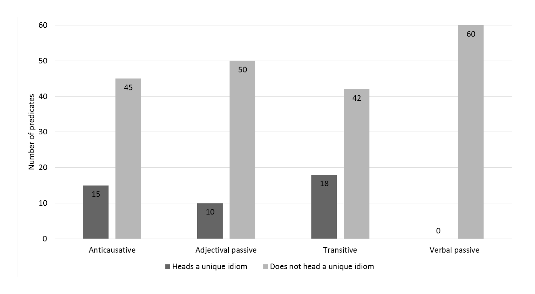
\includegraphics[width=\textwidth]{./img/20.1.eps}
    \begin{tikzpicture}
      \begin{axis}[
        axis lines*=left,
        enlarge y limits={abs=1cm,upper},
        height = .3\textheight,
        legend cell align=left,
        legend columns=2,
        legend pos=north west,
        legend style={font=\footnotesize,anchor=north},
        nodes near coords,
        nodes near coords style={font=\footnotesize},
        ticklabel style={font=\footnotesize},
        width  = \textwidth,
        xtick=data,
        xticklabels = {Anticausative, Adjectival passive, Transitive, Verbal passive},
        ybar,
        ylabel={\footnotesize Number of predicates},
        ylabel near ticks,
        ymax=60,
        ymin=0,
      ]
        \addplot [fill=black!70] coordinates {
          (0,15) (1,10) (2,18) (3,0)
        };
        \addlegendentry{Heads a unique idiom}
        \addplot [fill=black!30] coordinates {
          (0,45) (1,50) (2,42) (3,60)
        };
        \addlegendentry{Does not head a unique idiom}
      \end{axis}
    \end{tikzpicture}
\end{figure}

In sum, while the verbal passive\is{passive} cannot head unique phrasal \isi{idioms}, the
adjectival passive\is{passive}, anticausative and transitive can do so. Before turning to
the account we advance for these findings, we first discuss an experiment we
ran in order to further test this pattern of distribution, and establish the
significance of its results.

\section{Psycholinguistic evidence}\label{sec:20.3}\largerpage
\subsection{Prediction} %3.1 /

In order to further investigate the phenomenon of lack of phrasal \isi{idioms} unique
to the verbal passive\is{passive}, we ran an experiment aiming to examine speakers’
competence in the domain of idiom\is{idioms} distribution. We adopted the experimental
design put forth by \textcite{SilHorKluWex2018}, which tested competence based
on invented \isi{idioms} in order to circumvent speakers’ probable acquaintance with
idioms in their mother tongue. We composed \isi{idioms} in \ili{English} inspired by
existing \ili{Hebrew} \isi{idioms} and taught them to native \ili{English} speakers. After
learning and assimilating the new \isi{idioms}, participants were tested on their
intuitions about the likelihood of \isi{idioms} in the verbal passive\is{passive}, adjectival
passive and anticausative to share their idiomatic meaning with their
transitive alternant. Our prediction was as follows. If the findings discussed
in the previous section indeed represent a linguistic pattern, then the
experiment should show a significant difference between the verbal passive\is{passive} and
the other diatheses regarding their likelihood, as perceived by native
speakers, to head unique \isi{idioms}.

\subsection{Participants and method}\largerpage[2.6] %3.2 /

Participants included 36 native \ili{English} speakers, 28 female and eight male.
33 were monolingual while three were bilingual with a native or native-like
knowledge of Bengali, \ili{Russian} and \ili{Spanish} (self-proclaimed). Their
ages ranged be\-tween 18 and 32 (mean age 21.6).  All participants had at least
13 years of education.  None had linguistic education concerning the subject
matter of this study.  Participants were recruited in class or via recruitment
ads and consisted of American students at MIT, Brown University and Wellesley
(MA) College. After participating in the experimental sessions, participants
received a \$20 participation fee.

\subsubsection{Stimuli} 
We composed 12 \ili{English} \isi{idioms} inspired by existing
\ili{Hebrew} idioms: four headed by a verbal passive\is{passive} predicate,
four headed by an
adjectival passive\is{passive}, and four headed by an anticausative. All predicates had a
transitive alternant, and all \isi{idioms} had a plausible transitive version,
as judged by six speakers, and had no similar idiom\is{idioms} in \ili{English}. Adjectival
passive predicates were those formed by the suffix \emph{-en}, which disallows
a verbal reading (e.g. \emph{shaven}). Verbal passive\is{passive} predicates were formed
by dative\is{dative case} verbs, which allow formation of passives that are unambiguously
verbal.{\interfootnotelinepenalty=10000\footnote{\textcite{LevRap1986} put forward the \enquote{\glsdesc{SCG}}
    (\glsunset{SCG}\gls{SCG}), which states that an adjectival passive\is{passive} of a
    dative\is{dative case} verb is possible only if its formation involves externalization of
    the argument that is able to stand as the sole realized complement of the
    verb.  Externalization refers to the mechanism turning an internal argument
    of the input verb into the argument that the adjectival passive\is{passive} modifies or
    is predicated of.  Thus, for instance, the Theme of the verb \emph{sell}
    can be its sole complement (i) and therefore the adjectival passive\is{passive} in (ii)
    is possible. In contrast, the Goal cannot be the sole complement of
    \emph{sell} (iii); hence, the adjectival passive\is{passive} in (iv) is ruled out. It
    then follows that any expression of the form in (v) (where adjectival
    passive\is{passive} formation would violate the \gls{SCG}) can only be verbal.

   \ea[]{They sold the car.}
   \ex[]{The sold car.}
   \ex[*]{They sold the guy. (intended meaning: \enquote*{They sold the guy something.})}
   \ex[*]{the sold guy (intended meaning: \enquote*{the guy who was sold something})}
   \ex[]{\dots{} was sold something}
   \z}} The full list of invented \isi{idioms}, including their \ili{Hebrew}
    source of inspiration, interpretation, and example of usage, is given in
    \Cref{app-14:b} (Form 1).

\subsubsection{Design} 
The experiment proceeded in two sessions. In the first, 
\isi{idioms} were taught based on a list of \isi{idioms} including their
respective interpretations and examples of usage (henceforth: the teaching
session). In the second session the \isi{idioms} previously taught were reviewed, and
participants were asked to complete three questionnaires: first, a multiple-choice
comprehension questionnaire, second, a completion questionnaire, third, the
target questionnaire, in which participants were asked to rate the likelihood
that the transitive version of the \isi{idioms} exists (henceforth: the practice and
testing session). For instance, the (invented) anticausative idiom\is{idioms} \emph{drown
in the trash can} \REF{ex:20.18a} was associated with the interpretation in
\REF{ex:20.18b} and usage example in \REF{ex:20.19}.  The comprehension
task, the completion task and the experimental task for this idiom\is{idioms} are
given in \REF{ex:20.20}, \REF{ex:20.21}, and \REF{ex:20.22},
respectively. The comprehension task required choosing the correct response out
of three options: a literal interpretation (\ref{ex:20.1}) in~\eqref{ex:20.20}, the
idiomatic interpretation we associated with the idiom\is{idioms}
\eqref{ex:20.2}
in~\eqref{ex:20.20}, and a wrong (but contextually plausible) idiomatic
expression \eqref{ex:20.3} in~\eqref{ex:20.20}.

For all the \isi{idioms} used in the experiment see \Cref{app-14:b} (Form 1).

\ea\label{ex:20.18}
    \ea\label{ex:20.18a} drown in the trash can
    \ex\label{ex:20.18b} Interpretation: `get fooled'
    \z
\ex \label{ex:20.19}Usage example\\
    Alice really enjoys playing practical jokes on her friends and family. They
    are all pretty gullible, but her favorite victim is her little sister who
    somehow manages to drown in the trash can each and every time Alice tries
    to set her up.
\ex \label{ex:20.20}Comprehension
    \sn A: Why are you so angry?\\
        B: It's my annoying sister with her practical jokes.  I feel so stupid.
        This time she told me she got married in Vegas, and I was stupid enough
        to drown in the trash can and call every member of our family.
    \sn In the dialogue above, when B says \enquote{drown in the trash
        can}, she means that:
    \sn 1. She got so excited she walked right into a bin full of garbage\\
    \sn 2. She got fooled\\
    \sn 3. She got upset
\ex \label{ex:20.21}Completion\\
    Complete the following: She drowned in the \underline{\hphantom{3em}}
\ex \label{ex:20.22}Experimental task\\
    You have learned the idiom\is{idioms} `drown in the trash can'. How likely (from 1--5)
    does it seem to you that the following idiom\is{idioms} exists as well?
    \sn \enquote*{drown someone in the trash can}
\z

\subsubsection{Procedure} 
As mentioned above, the experiment included two
sessions. In the teaching session, the instructor first explained to the group
of participants that they were about to learn invented \isi{idioms} on which they
would be asked questions in a following meeting. The instructor then
distributed the list of idioms, interpretations and usage examples (Form 1, see
\Cref{app-14:b}), and taught the \isi{idioms} by reading each idiom\is{idioms} aloud in various
tenses (to assure participants do not assume their tense is fixed), along with
its meaning and example of usage. Participants were then asked to go over the
idioms again before the second meeting. The practice and testing session took
place three days later. The instructor made sure each participant had a copy of
Form 1 and slowly read its contents aloud. Participants were then asked to
return the form and were given the comprehension questionnaire (Form 2,
\Cref{app-14:b}), the completion questionnaire (Form 3, \Cref{app-14:b}), and the
experimental questionnaire on which participants rated the likelihood of an
idiom’s transitive version to exist (Form 4, \Cref{app-14:b}), printed side
down.  Participants were instructed to first fill in Forms 2 and 3, and only
then proceed to Form 4 (experimental questionnaire). The instructor made sure
this process was indeed executed in the specified order and that participants
did not look at a previous form once they continued on to the next one.

Data from one participant who had a total of three errors altogether in the two
practice forms were discarded, given that the task required assimilation of the
idioms. Data from six additional participants, who had one error altogether were
included, assuming that one error does not cast doubt on the speaker’s
knowledge of the learned \isi{idioms}.

\subsection{Results}  %3.3 /

\Cref{fig:20.2} shows the mean acceptance ratings of the transitive counterpart per diathesis.

\begin{figure}
    \caption{Mean acceptance ratings of transitive counterpart by diathesis
    (error bars represent standard deviation)}\label{fig:20.2}
    
    \begin{tikzpicture}
      \begin{axis}[
        axis lines*=left,
        bar width = 1cm,
        enlarge x limits=0.25,
        height = .3\textheight,
        width  = \textwidth,
        xtick=data,
        xticklabels = {Verbal passive, Anticausative, Adjectival passive},
        ybar,
        ymin=0,
      ]
        \addplot [fill=black!30,error bars/.cd, y dir=both, y explicit] coordinates {
          (0,4.33) +- (0.82,0.82)
          (1,3.19) +- (1.05,1.05)
          (2,2.44) +- (1.19,1.19)
        };
      \end{axis}
    \end{tikzpicture}
% %     
\includegraphics[width=.9\textwidth]{./img/20.2.eps}

\end{figure}

We used the lmerTest package in R \parencite{Kuzetal2015} to fit a mixed
effects model to our data, with ratings of the transitive version’s likelihood
as the dependent variable, diathesis of taught idiom\is{idioms} as the fixed factor, and
participants and items as random effects.

Following \citet{Barretal2013}, we started out by running a maximal model
including subject and item random intercepts and a random slope for the fixed
effect. Due to convergence failure, random slope was removed for items (but not
for subjects). This model yielded a significant effect of
diathesis\footnote{Test-statistics were obtained by the application of the
    functions ANOVA (for $F$ and $p$ values evaluating the role of the fixed
    factor as a predictor) and \emph{difflsmeans} (for estimates, labeled as
\emph{β}, standard errors and $t$ and $p$ values evaluating the
difference between conditions).} ($F(2,14.9) = 13.77$, $p < 0.001$).

As shown in \Cref{tab:20.3}, planned pairwise comparisons with an
application of a Bonferroni correction for multiple comparisons (X3) revealed
that ratings for transitive counterparts of \isi{idioms} headed by a verbal passive
(M = 4.33, SD = 0.82) were significantly higher than ratings of transitive
counterparts of \isi{idioms} headed by anticausatives (M = 3.19, SD = 1.05) and that
ratings for transitive counterparts of \isi{idioms} headed by anticausatives were
significantly higher than those provided for the transitive counterparts of
idioms headed by an adjectival passive\is{passive}  (M = 2.44, SD = 1.19).

\begin{table}
\caption{Planned pairwise comparisons between diathesis of
taught idiom}\label{tab:20.3}
\begin{tabularx}{\textwidth}{Qrrrr}
\lsptoprule
    & $B$ & {SE} & \multicolumn{1}{c}{$t$(df)} & $p$-value (corr.)\\
\midrule
{verbal passive/anticausative} & 1.0 & 0.26 & \emph{t}(16.8) = 3.96 & 0.003 \\
{verbal passive/adjectival passive} & 1.7 & 0.32 & \emph{t}(27) = 5.22 & $<0.001$\\
{anticausative/adjectival passive} & 0.7 & 0.24 & \emph{t}(13.2) = 2.78 & 0.045\\
\lspbottomrule
\end{tabularx}
\end{table}

In sum, the transitive counterparts of verbal passive\is{passive} \isi{idioms} were rated as
significantly more likely to exist than those headed by anticausatives and
adjectival passives. In addition, unlike in the \ili{Hebrew} experiment, the
transitive alternants of anticausative \isi{idioms} were rated as significantly more
likely to exist than those of \isi{idioms} headed by adjectival passives.

\section{Discussion}\label{sec:20.4} %4. /

\subsection{Support for Horvath \& Siloni’s approach}  %4.1 /

The survey of \ili{English} idiom\is{idioms} dictionaries has shown that phrasal idioms
distribute differently in the verbal passive\is{passive} diathesis versus the transitive,
anticausative and adjectival passive\is{passive} diatheses: while they cannot be unique to
the verbal passive\is{passive}, they can be unique to the latter diatheses. The experiment
we conducted further supports this pattern of distribution: participants
perceived the likelihood of the verbal passive\is{passive} to share idiomatic meanings with
its transitive counterpart as significantly higher than that of both the
adjectival passive\is{passive} and the anticausative. That is, the likelihood of the verbal
passive to head unique \isi{idioms} is significantly lower than that of the two other
diatheses. Both the survey and the experiment reveal that the distribution of
idioms is sensitive to the diathesis of their respective head.  This
sensitivity reinforces the claim that \isi{idioms} are stored as linguistic knowledge
(i.e., intra-grammatically), since otherwise there would be no reason for them
to be affected by a grammatical factor such as the diathesis of their
head.\footnote{As observed by \textcite{SilHorKluWex2018}, one could suggest that
    the learnt \isi{idioms} in the experiment were not stored in the participants'
    lexicon, as would be assumed under circumstances of natural learning, but
    rather placed in some short term storage, given that the exposure and
    learning take place in an experimental setting. A priori, this could be a
    possible alternative hypothesis.  However, this short term storage would by
    assumption be outside the grammar’s storage component. Thus, adopting this
    hypothesis would leave us with the question of why the results of the
    experiment turn out to pattern the way they do and specifically why they
    manifest sensitivity to diathesis. The short-term storage hypothesis in
    itself does not offer any account of the pattern of behavior revealed in
    the experiment. Moreover, the fact that the findings reproduced the pattern
    revealed by the survey of (existing) \isi{idioms} would then be a coincidence. }

Further, the existence of unique \isi{idioms} in the transitive, anticausative, and
adjectival passive\is{passive} shows that \isi{idioms} are not stored in the lexicon under the
root of their head, i.e., as subentries of the bare root. If they were, we
would erroneously predict prevalent idiom\is{idioms} sharing across diatheses, that is,
idiomatic meanings would have to be shared by the various diatheses generated
by the same root (under which \isi{idioms} would be stored), except for gaps due to
independent reasons. Likewise, if phrasal \isi{idioms} were stored under the root of
their head, all other things being equal, we would erroneously expect the
anticausative, adjectival passive\is{passive}, and verbal passive\is{passive} to be conceived by
speakers as equally likely to share idiomatic meanings with their transitive
alternants. (Recall that the transitive alternants of the experimental items
were judged as potentially possible \isi{idioms}.)

Following \textcite{HorSil2009,HorSil2019}, we derive the distributional
distinction between the verbal passive\is{passive} and the other diatheses, as revealed by
both the survey and the experiment, from the distinct storage technique
available to them. Consider first the options mentioned in the literature as to
how \isi{idioms} are stored. On the one hand, it has been suggested that \isi{idioms} are
stored as independent (``big'') lexical entries (e.g., in psycholinguistic
studies by \citealt{BobBel1973,SwiCut1979,Gibbs1980}). On the other hand, the
idea that \isi{idioms} are stored as subentries of other existing entries has also
been entertained: it has been suggested that they are stored by multiple
storage, that is, as subentries of the lexical entries of each of their
constituents \citep{Everaert2010}, or as subentries of the Encyclopedic entries
of their constituents (\citealt{HarNoy1999}). It has also been proposed that
they are stored under the lexical entry of the head of the idiom\is{idioms} only
\parencite{Baltin1989,HorSil2009}.\footnote{Analyses of \isi{idioms} claiming that
    the head of the idiom\is{idioms} selects the other subparts of the idiom\is{idioms} via a
    dependency between heads are common in earlier literature, and include a
    variety of otherwise different approaches, such as \citet{Bresnan1982},
    \citet{Erbach1992}, \citet{KooSpo1991}, and \citet{OGrady1998}.  These
    studies do not address the manner of storage, and are thus not explicit as
    to whether they propose that \isi{idioms} are listed exclusively as subentries of
    the entry of their head.  Yet based on their emphasis on head-on-head
    dependency and the parallels between their accounts of \isi{idioms} and other
    instances of ``selection''/``subcategorization'' (in the terminology of
    \citegen{Chomsky1965} Aspects model), it is reasonable to assume that these
proposals implicitly adopt a head-based storage for \isi{idioms} as well.}

\textcite{HorSil2009,HorSil2019} observe that the sensitivity of \ili{Hebrew}
phrasal \isi{idioms} to the diathesis of their head can be accounted for under the
assumption that they are stored as subentries of their head.\footnote{
    \textrm{The question as to whether there are good reasons to believe that
        they are stored in addition under the heads of the other constituents
in the idiom\is{idioms} is orthogonal to our discussion and will not be examined here.} }
If they were stored as independent entries of their own, there would be no
reason why their ability (in case of existing \isi{idioms}) and likelihood (in case
of invented \isi{idioms}) to exist as unique \isi{idioms} should depend on the specific
diathesis of their head. They could be stored as entries independently of
whether their head is a verbal passive\is{passive} or a predicate in some other diathesis.
On the other hand, under the assumption that they are stored as subentries,
there must exist a lexical entry whose subentries they can be. Thus, if their
head turns out not to be a lexical entry, evidently they cannot be stored as
its subentries, as further explained directly.

In the linguistic literature, it is a widely held view that the verbal passive
is not formed in the lexical component, but is derived by the computational
system post-lexically (\citealt{BakJohRob1989}; \citealt{Collins2005};
\citealt{HorSil2008}; \citealt{Meltzer-Asscher2012}, among others).
Being a post-lexical output, the verbal passive\is{passive} is, reasonably, not stored in
the lexical component. It follows that the verbal passive\is{passive} cannot have
subentries. Hence, an idiom\is{idioms} in the verbal passive\is{passive} cannot be stored directly
under the entry of its head, and thus cannot be unique to the diathesis. A
verbal passive\is{passive} idiom\is{idioms} must share its idiomatic meaning with its transitive
version, which is stored under the transitive entry. Post-lexical passivization
of the transitive idiom\is{idioms} is what produces the verbal passive
version.\footnote{We, correctly, do not predict the automatic existence of a
    verbal passive\is{passive} version for every transitive idiom. Since verbal passives
    are derived post-lexically, the question of whether or not a transitive
    idiom will exist in the verbal passive\is{passive} depends on whether the
    idiom\is{idioms} is able to undergo passivization resulting in a
    well-formed output.  This in turn involves interpretive factors, such as
    whether the idiom\is{idioms} chunk to become the derived subject of the
    passivized idiom\is{idioms} has the appropriate properties, e.g.,
    referentiality, to be compatible with the information structure
consequences of being in subject position (for discussion, see
\citealt{Ruwet1991}). See also \citet{NunSagWas1994} for discussion of the
question of which \isi{idioms} in the active can be passivized.}

Under \citeauthor{HorSil2009}'s (\citeyear{HorSil2009,HorSil2019}) approach,
the transitive, unaccusative\is{unaccusativity} (in our present terminology,
anticausative), and adjectival passive\is{passive}, unlike the verbal passive\is{passive}, are entries
in the lexicon. It then follows that an idiom\is{idioms} may be stored under each of them,
thereby enabling the existence of \isi{idioms} unique to the diathesis. Whether
or not these diatheses are indeed lexical entries is debated. But there are
studies advocating this claim on independent grounds. \citet{HorSil2011} and
\citet{Reinhart2002} argue that transitives are lexical entries, which can be
the input for additional diathesis derivations. Further, there are studies
claiming that unaccusatives and adjectival passives are derived by a lexical
operation (see \citealt{Chierchia2004}; \citealt{HorSil2011};
\citealt{LevRapHov1995}; \citealt{Koontz-Garboden2009}; \citealt{Reinhart2002},
for unaccusatives, and \citealt{HorSil2008}; \citealt{LevRap1986};
\citealt{Meltzer-Asscher2011}, for adjectival passives). Assuming with
\textcite{HorSil2008,HorSil2011} that these lexical outputs are stored in the
lexicon (more generally, that the adjectival passive\is{passive} and anticausative are
lexical entries), it becomes clear why they can have unique \isi{idioms}. Being
lexical entries, they can have their own subentries including \isi{idioms}
unique to them.

If indeed these diatheses are derived by lexical operations, it means that the
lexicon must be an active component of grammar (as argued by
\citealt{Reinhart2002}, \citealt{Siloni2002} among others), and not a mere
storehouse of atomic items, in contrast with the view of syntacticocentric
approaches (\citealt{Borer2005}; \citealt{Marantz1997};
\citealt{Pylkkanen2008}; \citealt{Ramchand2008}, among many others).

Recall, in addition, that the transitive alternants of anticausative idioms
were rated in the \ili{English} experiment as significantly more likely to exist than
the transitive alternants of those headed by adjectival passives. Obviously,
the transitive and adjectival passive\is{passive} differ in category (verbal vs.
adjectival, respectively), unlike the transitive and anticausative, which are
both verbal. One could then suggest that when sharing across diatheses involves
a change in lexical category, participants perceived it as less likely to
exist. However, the findings regarding \ili{Hebrew} cast doubt on this
suggestion, as such a distinction was not found in the \ili{Hebrew} experiment,
where the adjectival passive\is{passive} and the anticausative showed no significant
difference regarding the likelihood to share a transitive alternant. Moreover,
such significant effect between the anticausative and adjectival passive\is{passive} was
not found in the \ili{English} survey either. And, in fact, the number of adjectival
passives heading shared \isi{idioms} (21/60) in \ili{English} is even a bit larger than the
number of anticausatives heading shared \isi{idioms} (17/60). That is, there does not
seem to be a systematic distinction between the ability and likelihood of the
adjectival passive\is{passive} to share \isi{idioms} with the transitive and those of the
anticausative. We thus leave this issue open for further experimentation.

In sum, assuming that (i) the verbal passive\is{passive} is not stored in the lexicon
(since it is formed post-lexically), unlike the other diatheses, and (ii)
phrasal \isi{idioms} are stored as subentries of their head, the distinct
distribution of phrasal \isi{idioms} across diatheses follows. The verbal passive\is{passive},
unlike the other diatheses, cannot head unique \isi{idioms} as such \isi{idioms} would be
unable to be stored, given that the verbal passive\is{passive} is not a lexical entry.

This approach indeed accounts for the findings. But other approaches seem a
priori plausible too. We examine them in the next section.

\section{Alternative approaches}\label{sec:20.5} %4.2 /

As observed by \textcite{SilHorKluWex2018}, one might try to suggest that the
pattern revealed by the survey and experiment could be the reflection of the
productivity found at the diathesis level, that is, that the results reflect
inheritance from the verb level to the idiom\is{idioms} level. More specifically, the same
way that there are no verbal passives that lack a corresponding transitive
alternant, there are also no verbal passive\is{passive} \isi{idioms} that lack a transitive
counterpart. And the same way that there are sporadic gaps in the unaccusative
(anticausative) alternation – certain unaccusative\is{unaccusativity} verbs
idiosyncratically lack a transitive counterpart in a given language, and vice
versa – anticausative and transitive \isi{idioms} can similarly lack the
relevant alternant. Indeed, in the case of the verbal passive\is{passive}, an
approach of inheritance from the verb to the idiom level can be envisioned.
However, as far as the anticausative alternation is concerned, this approach is
implausible. While uniqueness at the idiom\is{idioms} level is a pervasive
phenomenon (as shown in \Cref{tab:20.2} and exemplified in
(\ref{ex:20.1}--\ref{ex:20.3}) and
(\ref{ex:20.9}--\ref{ex:20.11}) above),
unaccusative\is{unaccusativity} verbs systematically have a transitive
counterpart (with a Cause external role) and vice versa, except isolated
sporadic gaps \parencite{Haspelmath1993,Reinhart2002}.  Idiom distribution
across diatheses, therefore, cannot be considered to be a reflection of
productivity at the verb level.

A different potential account of the experimental findings could rely on the
difference in valence between verbal passives, which have two arguments
available (including the implicit\is{implicit arguments} external argument), versus anticausative and
adjectival passives, which are one-place predicates (but see~\cref{fn:20.16}). The
contrasting findings of the experiment may then follow, so the ``valence''
argument would go, from the fact that when participants are asked to estimate
the likelihood of the active transitive version based on a verbal passive
idiom, they are dealing with predicates of the same valence (both two-place),
while in case of having to relate an anticausative or an adjectival passive
idiom to a potential transitive version, participants need to convert a
one-place predicate into a two-place, transitive version of the same idiom. The
addition of an argument necessary in the anticausative and adjectival passive
cases but not in the verbal passive\is{passive} may add some extra difficulty to the task,
and thus it might be claimed to be the source of the difference in the results
found between these diatheses in the experiment. But such an approach would not
explain the total lack of unique verbal passive\is{passive} \isi{idioms} found in the surveys of
existing \isi{idioms} in both \ili{English} (\Cref{sec:20.2}) and \ili{Hebrew}
(\citealt{HorSil2009}). Suppose it is easier to “transitivize” a verbal passive
idiom, this still would not explain why the latter always has a transitive
alternant.\footnote{In addition, although in the past, it has been assumed that
    adjectival passives do not involve an implicit\is{implicit arguments} external argument, it was
    shown in recent literature that a subset of the set of adjectival passives
    does involve an external argument
    \parencite{Anagnostopoulou2003,GehMar2014,McIntyre2013,Meltzer-Asscher2011}.
    In the \ili{Hebrew} experiment, two adjectival passive\is{passive} \isi{idioms} are reported
    to be headed by an adjectival passive\is{passive} involving an external role
    (\emph{aruz} ‘packed’, \emph{tafur} ‘sewed’). These \isi{idioms} did not
        score better than the other two adjectival passive\is{passive} idioms
        \parencite{SilHorKluWex2018}. In the \ili{English} experiment the adjectival
passive \emph{shaven} implicates an external role. It did turn out to score
better. Thus, no conclusion can be drawn at this point.\label{fn:20.16}}

Within the framework of \isi{Distributed Morphology}, which has a single
struc\-ture-build\-ing engine, the syntax, \citet{Marantz1997} suggests that the
syntactic head introducing the external argument (Agent) is the boundary
delimiting the domain of special (idiomatic) meanings. He thus argues that the
fact that the verbal passive\is{passive} involves an external argument (explicit or
implicit)\is{implicit arguments} is the reason why it cannot be associated with special meanings (that
is, head unique \isi{idioms}). The unaccusative\is{unaccusativity}, in
contrast, lacks an external argument and can head unique \isi{idioms}. It is,
however, not obvious how this line of reasoning can account for the fact that
transitive verbs can head unique idioms, although they involve an external
argument (see also~\cref{fn:20.16}).\largerpage[2]

The syntactic boundary delimiting the domain for idiosyncratic meanings\linebreak could
then be argued to be higher than the head responsible for the Agent, say the
head responsible for the formation of verbal passives. The verbal
passive\is{passive} would not give rise to unique \isi{idioms} because it would
be beyond the syntactic domain of special meanings. Such a proposal would be at
odds with \citegen{Arad2005} arguments that the domain of idiosyncrasy is the
local domain of the root, and this is the domain delimited by the first
category-assigning head above the root; the domain of any higher head is argued
by Arad to have no access to meanings associated with the root. But if so, then
extending the locality domain, trying to cover the split behavior of
\isi{idioms} in the verbal passive versus the other diatheses we examined,
seems ad hoc.\footnote{Under some recent approaches dissociating Voice from
    \emph{v} (e.g., \citealt{Harley2013}), the passive\is{passive} Voice head
    merely captures the absence of the syntactic external argument (failure to
    merge a DP as its specifier) and is argued not to involve any of the
    particular semantics of the various ``flavors'' of \emph{v} (assumed by
    syntacticocentric approaches). Given such a proposal, one might perhaps
    think of attributing the absence of unique verbal passive\is{passive}
    \isi{idioms} to the Voice head’s lack of semantic substance. But the
    postulation of such a Voice head is not worked out in sufficient detail to
permit evaluation of its merits, and its potential ability to account for the
idiom\is{idioms} data.}

\section{Conclusion} %5. /

We have reported and discussed two novel empirical studies, one quantitative
survey of idiom dictionaries and one experimental study, examining the patterns
of distribution exhibited by phrasal \isi{idioms} across three diathesis alternations
in \ili{English}. The studies aimed to assess, based on evidence from two distinct
sources, what the cross-diathesis distribution of \isi{idioms} can tell us about
idiom storage, about the representation and derivation of these diatheses in
the grammar, and consequently about the division of labor between the lexicon
and the syntax.

Our investigation dealt with the question of whether there is an asymmetry in
the pattern of idiom distribution among the various diatheses, as reported in
the literature. Specifically, we investigated whether phrasal \isi{idioms} in the
verbal passive\is{passive} always have a transitive version, that is, cannot be unique to
the verbal passive\is{passive}, while the anticausative, adjectival passive\is{passive} and transitive
diatheses commonly exhibit \isi{idioms} specific to the diathesis. The results of our
English survey confirmed that the latter diatheses exhibit unique \isi{idioms}, while
the verbal passive\is{passive} always shares its idiomatic meaning with its transitive
alternant. The survey’s findings thus suggest that the distribution of phrasal
idioms depends on the particular diathesis of their head. To further confirm
these findings, which were based on the set of existing \isi{idioms}, we conducted
also an experimental study, which tested native speakers’ perception of the
likelihood of invented phrasal \isi{idioms} in the verbal passive\is{passive}, the adjectival
passive and the anticausative diathesis to share their idiomatic meaning with
their transitive alternant. The experimental results reproduced the same
pattern of asymmetric distribution as found in our idiom survey. Speakers
judged the likelihood of the verbal passive\is{passive} to share idiomatic meanings with
its transitive counterpart as significantly higher than the likelihood of the
other two diatheses.

The converging findings of these two different studies of the pattern of idiom
distribution were argued to follow from the particular storage technique
available to phrasal \isi{idioms}. Specifically, it was suggested that phrasal idioms
are stored in the lexicon as subentries of the entry of their head (not as
independent entries of their own). This proposal straightforwardly accounts for
the lack of unique phrasal \isi{idioms} in the verbal passive\is{passive}: Since the verbal
passive, unlike the other diatheses we examined, is a post-lexical output,
which does not have its own entry in the lexicon, it obviously cannot have
subentries. Hence, an idiom in the verbal passive\is{passive} cannot be stored directly
under its head, and thus cannot be unique to the diathesis. The transitive,
anticausative and adjectival passive\is{passive}, in contrast, are entries in the lexicon,
and can therefore list unique \isi{idioms} as their subentries. Our findings provide
evidence that the lexicon comprises derived diatheses as lexical entries,
rather than roots only. We take this as an indication that the lexicon is an
active component of grammar where derivational operations can apply.

\printchapterglossary{}

\section*{Acknowledgements}

This research was supported by Grant No.\ 2009269 from the United States–Israel
Binational Science Foundation (BSF). We would like to thank Kayla Gold-Shalev
for sampling the verbs and collecting the \isi{idioms} and Uriel Priva-Cohen for his
help with subject recruitment. Thanks also to two anonymous reviewers. Finally,
we are grateful to the editors of this volume for the opportunity to make a
contribution to this volume in honor of Ian Roberts.

{\sloppy
\printbibliography[heading=subbibliography,notkeyword=this]
}

\section*{Appendices}

In both the survey and the experiment, we took into account the notion of
decomposability first defined by \textcite{NunSagWas1994}. In their study of
idioms, \citeauthor{NunSagWas1994} distinguish between ``idiomatically combining
expressions'', in our terms, decomposable \isi{idioms}, and ``idiomatic expressions'',
in our terms nondecomposable \isi{idioms}. An idiom is considered decomposable if its
structure is isomorphic with its meaning, in the sense that its constituents
correspond to elements of its meaning. If not, it is nondecomposable.
\textcite{NunSagWas1994} claim that decomposability is a prerequisite for
``syntactic flexibility'', such as the ability of subparts of an idiom to
undergo movements.  If decomposability affects flexibility (movement), it seems
relevant for the shift between diatheses.

However, it must first be noted that the claim that decomposability is a
prerequisite for the syntactic flexibility of \isi{idioms} is in fact a rather
controversial one. Counterexamples seem to be frequently attested; for
instance, the following nondecomposable \isi{idioms}, which nonetheless exhibit
diathesis alternation: \emph{break someone’s heart} ‘sadden, disappoint
someone’, \emph{open the door to something} ‘enable, allow something to
happen', which both have an unaccusative counterpart, and \emph{keep tabs}
‘observe, follow’, which has a verbal and adjectival passive\is{passive}
counterpart.

Nonetheless, to be on the safe side, we did try to take this claim into
consideration and chose \isi{idioms} in our survey as well as \isi{idioms} for the
experiment so as to avoid this potentially interfering factor. Our guidelines
were as follows. In cases where the lexically fixed subparts would be involved
in the relevant diathesis changing operation, we included \isi{idioms} only if their
meaning (interpretation) could be mapped onto their head and its arguments (or
modifiers). We did not consider metaphoric paraphrases as interpretations
appropriate to determine decomposability. In addition, we did not consider it
relevant to have matching between parts of meaning and elements of the internal
structure of arguments (or modifiers). For instance, the idiom \emph{burn
one’s boats/bridges} (item 1, list of unique transitive \isi{idioms}) as well as
\emph{one’s red bulb lit up} (item 5, Form 1 of the experiment, \Cref{app-14:b})
are considered decomposable (as schematized here: [\tss{1} \emph{burn}]
[\tss{2} \emph{one’s boats/bridges}] ‘[\tss{1} destroy] [\tss{2} options of
reversing the situation]’; [\tss{1} \emph{one’s red bulb}] [\tss{2} \emph{lit
up}] ‘[\tss{1} one’s suspicion] [\tss{2} arose]’). Nondecomposable \isi{idioms} were
freely used when the potential diathesis shift operation would not involve a
lexically fixed constituent of the idiom, as for example in \emph{glued to
one’s seat}\slash \#\emph{glue one to one’s seat} (item 6, list of unique
adjectival passive\is{passive} \isi{idioms}, \Cref{app-14:a}).\largerpage[1]

\appendixsection{Survey}\label{app-14:a}
\largerpage
{\small
\begin{longtable}{ *{4}{>{\raggedright\arraybackslash}p{.25\linewidth - 2\tabcolsep}} }
\caption{Sampled predicates}\\
\lsptoprule Transitive  & Unaccusative & Adjectival passive & Verbal passive\\\midrule\endfirsthead
\midrule Transitive  & Unaccusative & Adjectival passive & Verbal passive\\\midrule\endhead
\endfoot\lspbottomrule\endlastfoot
bend      & bend      & beaten     & baked\\
blacken   & blacken   & bent       & bashed\\
blur      & blur      & bitten     & basted\\
bounce    & bounce    & blackened  & bathed\\
break     & break     & blasted    & beaten\\
brighten  & brighten  & blended    & bent\\
burn      & burn      & blessed    & bitten \\
burst     & burst     & bloated    & blackened\\
chafe     & chafe     & blocked    & blamed\\
change    & change    & blurred    & blended\\
chill     & chill     & bombed     & blinded\\
clear     & clear     & borrowed   & blocked\\
close     & close     & bottled    & boiled\\
cool      & cool      & bound      & bought\\
crack     & crack     & brightened & branded\\
crumble   & crumble   & broken     & brightened\\
curl      & curl      & built      & brought\\
dampen    & dampen    & buried     & bruised\\
darken    & darken    & caged      & built \\
deepen    & deepen    & carved     & burned\\
defrost   & defrost   & caught     & buttered\\
dim       & dim       & charged    & caged\\
drown     & drown     & charmed    & called\\
dry       & dry       & chilled    & cancelled \\
empty     & empty     & cleaned    & capped\\
evaporate & evaporate & cleared    & carried\\
explode   & explode   & clipped    & carved\\
flatten   & flatten   & clogged    & cashed\\
float     & float     & closed     & caught\\
freeze    & freeze    & cooked     & chewed\\
harden    & harden    & crushed    & chosen\\
heal      & heal      & cut        & closed\\
heat      & heat      & darkened   & cooked\\
improve   & improve   & destroyed  & counted\\
increase  & increase  & eaten      & cut\\
loosen    & loosen    & examined   & driven\\
melt      & melt      & fed        & dropped\\
move      & move      & fried      & frozen\\
narrow    & narrow    & glued      & given\\
open      & open      & joined     & handed\\
redden    & redden    & loaded     & hit\\
roll      & roll      & locked     & kept\\
shatter   & shatter   & marked    & kicked\\
shrink    & shrink    & packed    & left\\
shut      & shut      & painted   & lifted\\
sink      & sink      & poisoned  & painted\\
soften    & soften    & restored  & played\\
spill     & spill     & scared    & pulled\\
spin      & spin      & shaven    & pushed\\
split     & split     & shut      & robbed\\
spread    & spread    & stolen    & rubbed\\
stiffen   & stiffen   & stripped  & sent\\
stop      & stop      & stuffed   & shaken\\
suffocate & suffocate & sunken    & sold\\
thaw      & thaw      & taken     & stuffed\\
thicken   & thicken   & tied      & swept\\
tighten   & tighten   & varnished & taken\\
weaken    & weaken    & whitened  & thrown\\
worsen    & worsen    & wrapped   & wrapped\\
wrinkle   & wrinkle   & written   & written\\
\end{longtable}}
\largerpage
% % \subsection{Unique unaccusative idioms}\relax\is{unaccusativity}
\begin{table}[H]
\small
\caption{Unique unaccusative idioms}
\begin{tabularx}{\textwidth}{llQ}
\lsptoprule
{Verb} & {Idiom} & {Interpretation} \\
\midrule
{1. bend}  & bend in the wind & ‘be adaptable to difficulties’\\
{2. bounce}  & bounce off the walls & ‘be in a nervous and confused condition, be hyper’\\
{3. break}  & break even & ‘neither gain nor lose any money’, ‘recoup the money one invested’\\
{4. burn}  & burn with a low blue flame & ‘be quietly and intensely angry’, ‘be heavily intoxicated with alcohol’ \\
{5. burst}  & burst at the seams & ‘be extremely full or crowded’  \\
{6. chafe}  & chafe at the bit & ‘be impatient and/or eager for something to happen’\\
{7. crack}  & crack under the strain & ‘have a mental or emotional collapse because of continued work or stress’\\
{8.evaporate} & evaporate into thin air & ‘disappear quickly, without leaving a trace’\\
{9. explode}  & explode in one’s face & ‘unexpectedly fail, suddenly turn out to have’\\
{10. float}  & float on air & ‘be very happy and excited, feel euphoric’\\
{11. move}  & move up in the world & ‘advance and become successful’ \\
{12. roll}  & roll in the aisles & ‘laugh loudly’ \\
{13. sink} & sink through the floor & ‘suffer extreme embarrassment’\\
{14. spin}  & spin in one’s grave & ‘show enormous disfavor for something that has happened after one's death’\\
{15. thicken}  & the plot thickens & ‘the situation becomes more complicated\slash  interesting’\\
\lspbottomrule
\end{tabularx}
\end{table}

% % \subsection{Unique transitive idioms}\relax
\begin{table}[H]
\small
\caption{Unique transitive idioms}
\begin{tabularx}{\textwidth}{llQ}
\lsptoprule
{Verb} & {Idiom} & {Interpretation} \\
\midrule
{1. burn}  & burn one’s boats/bridges & ‘destroy options of reversing a situation’ \\
{2. burst}  & burst a blood-vessel & ‘use a lot of effort (doing…)’\\
{3. change} & change one’s stripes~ & ‘switch one’s opinion/ideology’ \\
{4. chill}  & chill one’s action & ‘discourage/disrupt one’s progress \\
{5. clear}  & clear the air & ‘eliminate doubts/hard feelings’\\
{6. crack}  & crack the case & ‘solve the crime/the problem’ \\
{7. drown}  & drown one’s sorrows & ‘suppress-by-drinking feeling of sadness\\
{8. empty}  & empty the tank & ‘contribute/expend the utmost of one’s energy’ \\
{9. move}  & move heaven and earth & ‘make a huge effort’ \\
{10. open}  & open the/one’s kimono & ‘reveal what one is planning’\\
{11. roll}  & roll the dice & ‘take a chance (on something)’ \\
{12. sink}  & sink one’s teeth into \dots & ‘undertake an endeavor for \dots’\\
{13. soften}  & soften the blow & ‘ease a difficult experience’ \\
{14. spill}  & spill the beans & ‘disclose a secret’ \\
{15. spin}  & spin one’s wheels & ‘waste time’\\
{16. split}  & split one’s sides & ‘laugh very hard’\\
{17. spread}  & spread one’s wings & ‘start new and different things’  \\
{18. tighten} & tighten one’s belt & ‘exercise/adopt thrift/frugality’\\
\lspbottomrule
\end{tabularx}
\end{table}

% % \subsection{Unique adjectival passive\is{passive} idioms}\relax
\begin{table}[H]
\is{passive}
\small
\caption{Unique adjectival passive idioms}
\begin{tabularx}{\textwidth}{llQ}
\lsptoprule
{Predicate} & {Idiom} & {Interpretation}\\
\midrule
{1. bent}     & {bent on a splice}                             & ‘be about to get married’\\
{2. built}    & {built like a tank}                            & ‘have a physique that is strong and physically imposing’\\
{3. caught}   & {caught in the middle}                         & ‘be between two opposing sides’ \\
{4. cut}      & {cut and dried}                                & ‘easy to see or understand the truth’ \\
              & {cut from the same cloth}                      & ‘of the same nature, similar’ \\
{5. fed}      & {fed to the gills\slash fed to the (back) teeth } & ‘disgusted, unable or unwilling to put up with something’ \\
{6. glued}    & {glued to one’s seat}                          & ‘to be extremely interested in something or so involved with something that you cannot move’\\
{7. joined}   & {joined at the hip}                            & ‘very closely connected, always together’\\
{8. loaded}   & { loaded for bear}                             & ‘eager/ready for a fight, angry’\\
{9. tied}     & { tied to one’s mother’s apron strings}        & ‘dependent on/dominated by one’s mother’ \\
{10. written} & { written in stone}                            & ‘fixed/unchangeable’ \\
\lspbottomrule
\end{tabularx}
\end{table}

\clearpage
\appendixsection{Forms}\label{app-14:b}

\appendixsubsection{Form 1}

Idioms\is{idioms}, interpretations and usage examples (the copies distributed
to participants did not include indications of diatheses)

{\small
\begin{longtable}{ l@{ } >{\raggedright}p{\widthof{stained under his/her skin}} >{\raggedright}p{\widthof{Interpretation}}  >{\raggedright\arraybackslash}p{ \linewidth - 6\tabcolsep - \widthof{~} - \widthof{stained under his/her skin} - \widthof{Interpretation}} }
\caption*{Form 1: \isi{idioms}, interpretations and usage examples (the copies distributed to participants did not include indications of diatheses)}\\
\lsptoprule & Idiom  & Interpretation & Usage example\\\midrule\endfirsthead
\midrule & Idiom  & Interpretation & Usage example\\\midrule\endhead
\endfoot\lspbottomrule\endlastfoot
1. & \textbf{was sold a stew of lentils} \newline
   (verbal passive) \newline
   Inspiring \ili{Hebrew} idiom: \newline
   \textbf{\emph{maxar et \emph{x} be-nezid\newline adašim}} \newline
   sold \Acc{} \emph{x} in stew\newline lentils \newline
   \enquote*{accepted a bad deal} & was deceived & Danny hates going out in the middle of the week because he has to get up early in the morning. That's the reason he was very reluctant to attend his friends' midweek party. But when they told him Sara, the girl he liked so much, was going to be there, he accepted the invitation. When he got to the party, he waited impatiently for her to arrive, but she never showed up. Only then did he realize that he was sold a stew of lentils. His friends probably didn't even invite Sara. They were only trying to get him to come to the party.\\
2. & \textbf{stained under his/her skin} \newline
   (adjectival passive) \newline
   Inspiring \ili{Hebrew} idiom: \newline
   \emph{\textbf{rakuv mi-befnim}} \newline
   rotten from inside\newline
   \enquote*{corrupt (human being)} & secretly corrupt & Dina was the only one who wasn't surprised to hear that the chair of the tenants' board embezzled the building's funds. Unlike everyone else, who admired his character, she always considered him to be one of those types who seem stained under their skin.\\
3. & \textbf{warm up in one's light} \newline
   (unaccusative) \newline
   Inspiring \ili{Hebrew} idiom: \newline
   \emph{\textbf{hitxamem le-or-\emph{x}}} \newline
   warmed.up to-light-\emph{x}\newline
   \enquote*{learned/benefited from\newline someone's knowledge} & benefit
   from\newline one's knowledge & The first person Lisa thanked in the acknowledgments part of her dissertation was her thesis advisor Professor Green. After all, Lisa has warmed up in his light ever since she was an undergrad.\\
4. & \textbf{sunken in a pit of lard} \newline
   (adjectival passive) \newline
   Inspiring \ili{Hebrew} idiom: \newline
   \textbf{\emph{(haya) be-kluv šel zahav}} \newline
   (was) in-cage of gold\newline
   \enquote*{was in a comfortable\newline but
   limiting/damaging\newline situation} &
   trapped in a comfortable but damaging situation & John married Maggie at a very young age, and since she was a very rich and successful business woman, he never had to pursue a demanding career. But now, sitting by the pool all day at age 39 with no purpose, it is  pretty obvious he is sunken in a pit of lard.\\
5. & \textbf{one's red bulb lit up} \newline
   (unaccusative) \newline
   Inspiring \ili{Hebrew} idiom: \newline
   \textbf{\emph{nidleka le-\emph{x} nura}} \newline
   lit.up to-\emph{x} bulb red\newline
   \enquote*{one's suspicion arose} & one's suspicion arose & David wasn't very surprised when he got fired; he had already suspected this was about to happen. His red bulb lit up when he asked his boss if he should order a new office chair and couldn’t get a straight answer.\\
6. & \textbf{was handed soggy bread} \newline
   (verbal passive) \newline
   Inspiring \ili{Hebrew} idiom: \newline
   \textbf{\emph{he'exil et \emph{x} be-lokšim}} \newline
   fed \Acc{} \emph{x} in-noodles\newline
   \enquote*{told someone false stories} & was told a fib in order ot
                                         keep him quiet & Shelly and Andy have been dating for almost two years and recently moved in together. A week after they moved, Shelly's grandfather decided to come for a visit. Shelly knew that if her conservative grandfather finds out they have no plans of ever getting married, he will not stop complaining about it; she decided to avoid this and came up with a ploy. When grandpa arrived he was handed soggy bread by the two of them: they happily announced they were engaged to be married.\\
7. & \textbf{drown in the trash can} \newline
   (unaccusative) \newline
   Inspiring \ili{Hebrew} idiom: \newline
   \textbf{\emph{nafal ba-pax}} \newline
   fell in.the-bin\newline
   \enquote*{got fooled} & get fooled & Alice really enjoys playing practical jokes on her friends and family. They are all pretty gullible, but her favorite victim is her little sister who somehow manages to drown in the trash can each and every time Alice tries to set her up. \\
8. & \textbf{break out of his/her harness} \newline
   (unaccusative) \newline
   Inspiring \ili{Hebrew} idiom: \newline
   \textbf{\emph{yaca me-ha-kelim}} \newline
   got.out from-the-tools/\newline equipment\newline
   \enquote*{lost one's temper} & get angry & Being a 2{nd} grade teacher, Rachael knows it's very important that she stays calm even when her students act out. But when one of the kids spilled glue all over her designer shoes, she broke out of her harness and screamed at him.\\
9. & \textbf{stricken with tremors} \newline
    (adjectival passive) \newline
    Inspiring \ili{Hebrew} idiom: \newline
    \textbf{\emph{axuz palacut}} \newline
    caught horror\newline
    \enquote*{terrorized} & frantic & Lisa's son really likes his babysitter. At first, Lisa thought it's because he likes playing with her, but after the third time she returned home to a boy stricken with tremors and unable to go to sleep, she gathered that the reason for his affection for this girl is that she gives him all the candy he asks for.\\
10. & \textbf{shaven on both sides of his/her face} \newline
   (adjectival passive) \newline
   Inspiring \ili{Hebrew} idiom: \newline
   \textbf{\emph{megulax mi-kol kivun}} \newline
   shaven from-all-direction\newline
   \enquote*{left with nothing, lost everything} & left with nothing & When Lisa decided to start looking for a better job, she thought that going to job interviews on her lunch breaks was a good idea. But these long lunches she took led to her being fired from her current job. Now she is shaven on both sides of her face with no job at all.\\
11. & \textbf{was slipped the smudge} \newline
   (verbal passive) \newline
   Inspiring \ili{Hebrew} idiom: \newline
   \textbf{\emph{hetil bo dofi}} \newline
   throw in.him fault\newline
   \enquote*{doubted him, spoke ill of him} & was maligned behind his
                                            back & At first, John had no idea who could have spread the nasty rumors about mice in his restaurant. But then he remembered how badly things ended with his head waiter a month ago, and realized that he was slipped the smudge by that angry former employee.\\
12. & \textbf{was given the heavy beam} \newline
            (verbal passive) \newline
            Inspiring \ili{Hebrew} idiom: \newline
            \textbf{\emph{nixnas be-ovi ha-kora}} \newline
            entered in-thickness the-beam\newline
            \enquote*{delved deeply into \dots{}} & was held responsible for
            the failure & Even though Johnny made pretty good money tutoring last year, he decided to never do it again. He took it pretty hard when one of his lazier students failed his exam and it was Johnny that was given the heavy beam by the kid's parents.\\
\end{longtable}
}
%\end{table}

%\begin{table}
%{\smaller
%%    \caption*{Form 1 (continued)}
%    \begin{tabularx}{\textwidth}{@{}lXXX@{}}
%%\lsptoprule
%& {\bfseries Idiom} & {\bfseries Interpretation}  & {\bfseries Usage example} \\
%\midrule
%%\textbf{10.} & \textbf{shaven on both sides of his/her face} \newline
%%            (adjectival passive) \newline
%%            Inspiring \ili{Hebrew} idiom: \newline
%%            \textbf{\emph{megulax mi-kol kivun}} \newline
%%            shaven from-all-direction\newline
%%            \enquote*{left with nothing, lost everything} & left with nothing & When Lisa decided to start looking for a better job, she thought that going to job interviews on her lunch breaks was a good idea. But these long lunches she took led to her being fired from her current job. Now she is shaven on both sides of her face with no job at all.\\
%%\textbf{11.} & \textbf{was slipped the smudge} \newline
%%            (verbal passive) \newline
%%            Inspiring \ili{Hebrew} idiom: \newline
%%            \textbf{\emph{hetil bo dofi}} \newline
%%            throw in.him fault\newline
%%            \enquote*{doubted him, spoke ill of him} & was maligned behind his
%%                                                     back & At first, John had no idea who could have spread the nasty rumors about mice in his restaurant. But then he remembered how badly things ended with his head waiter a month ago, and realized that he was slipped the smudge by that angry former employee.\\
%\textbf{12.} & \textbf{was given the heavy beam} \newline
%            (verbal passive) \newline
%            Inspiring \ili{Hebrew} idiom: \newline
%            \textbf{\emph{nixnas be-ovi ha-kora}} \newline
%            entered in-thickness the-beam\newline
%            \enquote*{delved deeply into \dots{}} & was held responsible for
%            the failure & Even though Johnny made pretty good money tutoring last year, he decided to never do it again. He took it pretty hard when one of his lazier students failed his exam and it was Johnny that was given the heavy beam by the kid's parents.\\
%%\lspbottomrule
%\end{tabularx}
%}
%%\end{table}

%\newpage

\newpage
\appendixsubsection{Form 2}

\subsubsection*{Comprehension questions}

\begin{description}[style=sameline,noitemsep]
\item[Participant no.:] \underline{\hphantom{3em}}
\item[Age:] \underline{\hphantom{3em}}
\item[Gender:] \underline{\hphantom{3em}}
\item[Native English speaker:] yes/no
\item[Are there any other languages you speak? If yes, name these languages and estimate your level of knowledge (poor/good/excellent/native-like):] \underline{\hphantom{3em}}
\end{description}

\subsubsection*{Please read the following dialogue between A and B and circle the correct answer.}
%\sn \textbf{Form 2}: comprehension questions
%\sn Participant no.: \underline{\hphantom{3em}}
%\sn Age: \underline{\hphantom{3em}}
%\sn Gender: \underline{\hphantom{3em}}
%\sn Native \ili{English} speaker: yes/no
%\sn Are there any other languages you speak? If yes, name these languages and estimate your level of knowledge (poor/good/excellent/native-like): \underline{\hphantom{3em}}
%\sn Please read the following dialogue between A and B and circle the correct answer.
\begin{enumerate}
    \item \begin{enumerate}[nosep,label=\Alph*:]
    \item So why do you want to break up with Mary?
    \item I think she's cheating on me. My red bulb lit up when she started wearing perfume to work.
    \end{enumerate} 
    In the dialogue above, when B says \enquote{my red bulb lit up}, he means that:
    \begin{enumerate}[label=\arabic*.,noitemsep]
        \item his heart broke
        \item he was so depressed that he sat in the dark with a flashlight
        \item his suspicion arose
    \end{enumerate}
    \item \begin{enumerate}[nosep,label=\Alph*:]
        \item What do you think about the new guy?
        \item I'm not sure. He works hard but I get really distracted sitting across from him, he is stricken with tremors all the time!
        \end{enumerate}
       In the dialogue above, when B says he \enquote{is stricken with tremors}, he means that:
       \begin{enumerate}[label=\arabic*.,noitemsep]
        \item he is sick
        \item he is frantic
        \item he is very chatty
        \end{enumerate}
    \item
        \begin{enumerate}[nosep,label=\Alph*:]
        \item So how is your son doing at school?
        \item Well, every evening after dinner he supposedly goes up to his room to study, but when I looked at his report card yesterday I realized I had been sold a stew of lentils.
        \end{enumerate}
        In the dialogue above, when B says she \enquote{was sold a stew of lentils}, she means that:
        \begin{enumerate}[label=\arabic*.,noitemsep]
        \item she was given the wrong bowl of soup
        \item she was deceived
        \item she received confidential news
        \end{enumerate}
    \item
       \begin{enumerate}[nosep,label=\Alph*:]
        \item Please don't fire me, I promise I’ll never be late again.
        \item You leave me no choice. You always say you arrive on time but on five different occasions customers called to complain that the store was closed for at least 45 minutes after opening time. I've been handed soggy bread again and again and I won't have it!
        \end{enumerate}
        In the dialogue above, when B says \enquote{I've been handed soggy bread}, she means that:
        \begin{enumerate}[label=\arabic*.,noitemsep]
        \item she was blamed for something she didn't do
        \item she was told a fib in order to keep her quiet
        \item she was yelled at by angry customers
        \end{enumerate}
    \item
        \begin{enumerate}[nosep,label=\Alph*:]
        \item How did your family dinner go yesterday?
        \item It went pretty smoothly until my granddad broke out of his harness when my brother used the wrong fork.
        \end{enumerate}
        In the dialogue above, when B says her granddad \enquote{broke out of his harness}, she means that:
        \begin{enumerate}[label=\arabic*.,noitemsep]
        \item he fell off his chair
        \item he laughed
        \item he got angry
        \end{enumerate}
    \item
       \begin{enumerate}[nosep,label=\Alph*:]
        \item So what about these two guys you were dating simultaneously?
        \item Don’t ask, they found out about each other and now I am shaven on both sides of my face.
       \end{enumerate}
        In the dialogue above, when B says \enquote{I am shaven on both sides of my face}, she means that:
        \begin{enumerate}[label=\arabic*.,noitemsep]
        \item she is embarrassed
        \item she is left with nothing
        \item she is bruised
        \end{enumerate}
    \item
       \begin{enumerate}[nosep,label=\Alph*:]
        \item A: So what happened between Jennifer and Mary?
        \item B: I don't know the details, but I heard Mary found out she was slipped the smudge by Jennifer and decided never to speak to her again.
        \end{enumerate}
        In the dialogue above, when B says Mary \enquote{was slipped the smudge}, he means that:
        \begin{enumerate}[label=\arabic*.,noitemsep]
        \item she was soiled by a splash of mud
        \item she was asked for a loan
        \item she was maligned behind her back
        \end{enumerate}
    \item
       \begin{enumerate}[nosep,label=\Alph*:]
        \item Can you help me bake a cake for Mom's birthday?
        \item No. I promised myself never to bake with you again, after that time you forgot to take the muffins out of the oven and I was given the heavy beam. You never do what you're supposed to!
        \end{enumerate}
        In the dialogue above, when B says he \enquote{was given the heavy beam}, he means that:
        \begin{enumerate}[label=\arabic*.,noitemsep]
        \item he was injured by bumping into a beam
        \item he was held responsible for the failure
        \item he had to solve the problem
        \end{enumerate}
    \item
       \begin{enumerate}[nosep,label=\Alph*:]
        \item So who do you think will get the promotion?
        \item I think Maggie will give it to Steve, her former assistant. He has warmed up in her light for many years, which makes him the person she trusts the most.
        \end{enumerate}
        In the dialogue above, when B says \enquote{he has warmed up in her light}, he means:
        \begin{enumerate}[label=\arabic*.,noitemsep]
        \item he has benefited from her knowledge
        \item he has enjoyed her warm office
        \item he has felt comfortable around her
        \end{enumerate}
    \item
       \begin{enumerate}[nosep,label=\Alph*:]
        \item How do you like your new apartment?
        \item It's great—at a very central location and only a block away from my work. But the downside is that since it's so close to everything, I get no exercise at all. So I guess I’m sunken in a pit of lard.
        \end{enumerate}
        In the dialogue above, when B says she is \enquote{sunken in a pit of lard}, she means that:
        \begin{enumerate}[label=\arabic*.,noitemsep]
        \item she is lazy
        \item she is trapped in a comfortable but damaging situation
        \item she is not a vegetarian
        \end{enumerate}
    \item
       \begin{enumerate}[nosep,label=\Alph*:]
        \item Look at this guy, he has such warm eyes!
        \item Don't even think about it. He sure looks like a decent guy but my friend dated him for a while so I heard a lot about him. He really seems stained under his skin.
        \end{enumerate}
        In the dialogue above, when B says he really seems “stained under his skin", she means he really seems:
        \begin{enumerate}[label=\arabic*.,noitemsep]
        \item sick
        \item unstable
        \item secretly corrupt
        \end{enumerate}
    \item
       \begin{enumerate}[nosep,label=\Alph*:]
        \item Why are you so angry?
        \item It's my annoying sister with her practical jokes. This time she told me she got married in Vegas, and I was stupid enough to drown in the trash can and call every member of our family.
        \end{enumerate}
        In the dialogue above, when B says \enquote{drown in the trash can}, she means that:
        \begin{enumerate}[label=\arabic*.,noitemsep]
        \item she got so excited she walked right into a bin full of garbage
        \item she got  fooled
        \item she got upset
        \end{enumerate}
\end{enumerate}

\appendixsubsection{Form 3}
\subsubsection*{Completion task}
    \begin{enumerate}[nosep]
        \item She was sold a stew of \underline{\hphantom{3em}}
        \item He seems stained under his  \underline{\hphantom{3em}}
        \item He has warmed up in her  \underline{\hphantom{3em}}
        \item She is sunken in a pit of  \underline{\hphantom{3em}}
        \item His \underline{\hphantom{3em}} bulb lit up
        \item She was handed   \underline{\hphantom{3em}}  bread
        \item She drowned in the  \underline{\hphantom{3em}}   \underline{\hphantom{3em}}
        \item He  broke out of his  \underline{\hphantom{3em}}
        \item He is stricken with  \underline{\hphantom{3em}}
        \item She is shaven on both  \underline{\hphantom{3em}}  of her face
        \item She was slipped the \underline{\hphantom{3em}}
        \item He was given the \underline{\hphantom{3em}} beam
    \end{enumerate}
\appendixsubsection{Form 4}

\subsubsection*{Experimental task}

\noindent Participant no: \underline{\hphantom{3em}}

\noindent Please answer the following questions:\vspace{.5\baselineskip}

\noindent 1.\ You have learned the idiom \enquote*{{break out of his/her harness}}.

\noindent How likely (from 1--5) does it seem to you that the following idiom
exists as well?\vspace{.5\baselineskip}

\noindent \enquote*{{break someone out of his/her harness}}\vspace{.5\baselineskip}

\noindent \begin{tabularx}{\textwidth}{XXXXX}
    1 & 2 & 3 & 4 & 5\\
    Unlikely & & & & Very likely\\
\end{tabularx}\vspace{1\baselineskip}

\noindent 2.\ You have learned the idiom \enquote*{{was slipped the smudge}}.

\noindent How likely (from 1--5) does it seem to you that the following idiom exists
    as well?\vspace{.5\baselineskip}

\noindent \enquote*{{slip someone the smudge}}\vspace{.5\baselineskip}

\noindent \begin{tabularx}{\textwidth}{XXXXX}
        1 & 2 & 3 & 4 & 5\\
        Unlikely & & & & Very likely\\
        \end{tabularx}\vspace{1\baselineskip}


\noindent 3.\ You have learned the idiom \enquote*{{drown in the trash can}}.

\noindent How likely (from 1--5) does it seem to you that the following idiom exists
    as well?\vspace{.5\baselineskip}

\noindent \enquote*{{drown someone in the trash can}}\vspace{.5\baselineskip}

\noindent \begin{tabularx}{\textwidth}{XXXXX}
        1 & 2 & 3 & 4 & 5\\
        Unlikely & & & & Very likely\\
        \end{tabularx}\vspace{1\baselineskip}


\noindent 4.\ You have learned the idiom \enquote*{{shaven on both sides of
    her/his face}}.

\noindent How likely (from 1--5) does it seem to you that the following idiom exists
    as well?\vspace{.5\baselineskip}

\noindent \enquote*{{shave someone on both sides of her/his face}}\vspace{.5\baselineskip}

\noindent \begin{tabularx}{\textwidth}{XXXXX}
        1 & 2 & 3 & 4 & 5\\
        Unlikely & & & & Very likely\\
        \end{tabularx}\vspace{1\baselineskip}

\noindent 5.\ You have learned the idiom \enquote*{{one's red bulb lit up}}.


\noindent How likely (from 1--5) does it seem to you that the following idiom exists
    as well?\vspace{.5\baselineskip}

\noindent \enquote*{{light up one's red bulb}}\vspace{.5\baselineskip}

\noindent \begin{tabularx}{\textwidth}{XXXXX}
        1 & 2 & 3 & 4 & 5\\
        Unlikely & & & & Very likely\\
        \end{tabularx}\vspace{1\baselineskip}

\noindent 6.\ You have learned the idiom \enquote*{{sunken in a pit of lard}}.

\noindent How likely (from 1--5) does it seem to you that the following idiom exists
    as well?\vspace{.5\baselineskip}

\noindent \enquote*{{sink someone in a pit of lard}}\vspace{.5\baselineskip}

\noindent \begin{tabularx}{\textwidth}{XXXXX}
        1 & 2 & 3 & 4 & 5\\
        Unlikely & & & & Very likely\\
        \end{tabularx}\vspace{1\baselineskip}

\noindent 7.\ You have learned the idiom \enquote*{{was given the heavy beam}}.

\noindent How likely (from 1--5) does it seem to you that the following idiom exists
    as well?\vspace{.5\baselineskip}

\noindent \enquote*{{give someone the heavy beam}}\vspace{.5\baselineskip}

\noindent \begin{tabularx}{\textwidth}{XXXXX}
        1 & 2 & 3 & 4 & 5\\
        Unlikely & & & & Very likely\\
        \end{tabularx}\vspace{1\baselineskip}

\noindent 8.\ You have learned the idiom \enquote*{{warm up in one's light}}.

\noindent How likely (from 1--5) does it seem to you that the following idiom exists
    as well?\vspace{.5\baselineskip}

\noindent \enquote*{{warm someone up in one's light}}\vspace{.5\baselineskip}

\noindent \begin{tabularx}{\textwidth}{XXXXX}
        1 & 2 & 3 & 4 & 5\\
        Unlikely & & & & Very likely\\
        \end{tabularx}\vspace{1\baselineskip}

\noindent 9.\ You have learned the idiom \enquote*{{was sold a stew of lentils}}.

\noindent How likely (from 1--5) does it seem to you that the following idiom exists
    as well?\vspace{.5\baselineskip}

\noindent \enquote*{{sell someone a stew of lentils}}\vspace{.5\baselineskip}

\noindent \begin{tabularx}{\textwidth}{XXXXX}
        1 & 2 & 3 & 4 & 5\\
        Unlikely & & & & Very likely\\
        \end{tabularx}\vspace{1\baselineskip}


\noindent 10.\ You have learned the idiom \enquote*{{stained under his/her
    skin}}.

\noindent How likely (from 1--5) does it seem to you that the following idiom exists
    as well?\vspace{.5\baselineskip}

\noindent \enquote*{{stain someone under his/her skin}}\vspace{.5\baselineskip}

\noindent \begin{tabularx}{\textwidth}{XXXXX}
        1 & 2 & 3 & 4 & 5\\
        Unlikely & & & & Very likely\\
        \end{tabularx}\vspace{1\baselineskip}


\noindent 11.\ You have learned the idiom \enquote*{{was fed soggy bread}}.

\noindent How likely (from 1--5) does it seem to you that the following idiom exists
    as well?\vspace{.5\baselineskip}

\noindent \enquote*{{feed someone soggy bread}}\vspace{.5\baselineskip}

\noindent \begin{tabularx}{\textwidth}{XXXXX}
        1 & 2 & 3 & 4 & 5\\
        Unlikely & & & & Very likely\\
        \end{tabularx}\vspace{1\baselineskip}


\noindent 12.\ You have learned the idiom \enquote*{{stricken with tremors}}.

\noindent How likely (from 1--5) does it seem to you that the following idiom exists
    as well?\vspace{.5\baselineskip}

\noindent \enquote*{{strike someone with tremors}}\vspace{.5\baselineskip}

\noindent \begin{tabularx}{\textwidth}{XXXXX}
        1 & 2 & 3 & 4 & 5\\
        Unlikely & & & & Very likely\\
        \end{tabularx}

%\begin{exe}

%    \sn \textbf{Form 4}: Experimental task
%    \sn Participant no: \underline{\hphantom{3em}}
%    \sn Please answer the following questions:
%    \sn 1.\ You have learned the idiom \enquote*{\textbf{break out of his/her
%    harness}}.
%    \sn How likely (from 1--5) does it seem to you that the following idiom exists
%    as well?
%    \sn \enquote*{\textbf{break someone out of his/her harness}}
%    \sn \begin{tabularx}{\textwidth}{XXXXX}
%        1 & 2 & 3 & 4 & 5\\
%        Unlikely & & & & Very likely\\
%        \end{tabularx}
%    \sn 2.\ You have learned the idiom \enquote*{\textbf{was slipped the smudge}}.
%    \sn How likely (from 1--5) does it seem to you that the following idiom exists
%    as well?
%    \sn \enquote*{\textbf{slip someone the smudge}}
%    \sn \begin{tabularx}{\textwidth}{XXXXX}
%        1 & 2 & 3 & 4 & 5\\
%        Unlikely & & & & Very likely\\
%        \end{tabularx}
%    \sn 3.\ You have learned the idiom \enquote*{\textbf{drown in the trash can}}.
%    \sn How likely (from 1--5) does it seem to you that the following idiom exists
%    as well?
%    \sn \enquote*{\textbf{drown someone in the trash can}}
%    \sn \begin{tabularx}{\textwidth}{XXXXX}
%        1 & 2 & 3 & 4 & 5\\
%        Unlikely & & & & Very likely\\
%        \end{tabularx}
%    \sn 4.\ You have learned the idiom \enquote*{\textbf{shaven on both sides of
%    her/his face}}.
%    \sn How likely (from 1--5) does it seem to you that the following idiom exists
%    as well?
%    \sn \enquote*{\textbf{shave someone on both sides of her/his face}}
%    \sn \begin{tabularx}{\textwidth}{XXXXX}
%        1 & 2 & 3 & 4 & 5\\
%        Unlikely & & & & Very likely\\
%        \end{tabularx}
%    \sn 5.\ You have learned the idiom \enquote*{\textbf{one's red bulb lit up}}.
%    \sn How likely (from 1--5) does it seem to you that the following idiom exists
%    as well?
%    \sn \enquote*{\textbf{light up one's red bulb}}
%    \sn \begin{tabularx}{\textwidth}{XXXXX}
%        1 & 2 & 3 & 4 & 5\\
%        Unlikely & & & & Very likely\\
%        \end{tabularx}
%    \sn 6.\ You have learned the idiom \enquote*{\textbf{sunken in a pit of lard}}.
%    \sn How likely (from 1--5) does it seem to you that the following idiom exists
%    as well?
%    \sn \enquote*{\textbf{sink someone in a pit of lard}}
%    \sn \begin{tabularx}{\textwidth}{XXXXX}
%        1 & 2 & 3 & 4 & 5\\
%        Unlikely & & & & Very likely\\
%        \end{tabularx}
%    \sn 7.\ You have learned the idiom \enquote*{\textbf{was given the heavy beam}}.
%    \sn How likely (from 1--5) does it seem to you that the following idiom exists
%    as well?
%    \sn \enquote*{\textbf{give someone the heavy beam}}
%    \sn \begin{tabularx}{\textwidth}{XXXXX}
%        1 & 2 & 3 & 4 & 5\\
%        Unlikely & & & & Very likely\\
%        \end{tabularx}
%    \sn 8.\ You have learned the idiom \enquote*{\textbf{warm up in one's light}}.
%    \sn How likely (from 1--5) does it seem to you that the following idiom exists
%    as well?
%    \sn \enquote*{\textbf{warm someone up in one's light}}
%    \sn \begin{tabularx}{\textwidth}{XXXXX}
%        1 & 2 & 3 & 4 & 5\\
%        Unlikely & & & & Very likely\\
%        \end{tabularx}
%    \sn 9.\ You have learned the idiom \enquote*{\textbf{was sold a stew of lentils}}.
%    \sn How likely (from 1--5) does it seem to you that the following idiom exists
%    as well?
%    \sn \enquote*{\textbf{sell someone a stew of lentils}}
%    \sn \begin{tabularx}{\textwidth}{XXXXX}
%        1 & 2 & 3 & 4 & 5\\
%        Unlikely & & & & Very likely\\
%        \end{tabularx}
%    \sn 10.\ You have learned the idiom \enquote*{\textbf{stained under his/her
%    skin}}.
%    \sn How likely (from 1--5) does it seem to you that the following idiom exists
%    as well?
%    \sn \enquote*{\textbf{stain someone under his/her skin}}
%    \sn \begin{tabularx}{\textwidth}{XXXXX}
%        1 & 2 & 3 & 4 & 5\\
%        Unlikely & & & & Very likely\\
%        \end{tabularx}
%    \sn 11.\ You have learned the idiom \enquote*{\textbf{was fed soggy bread}}.
%    \sn How likely (from 1--5) does it seem to you that the following idiom exists
%    as well?
%    \sn \enquote*{\textbf{feed someone soggy bread}}
%    \sn \begin{tabularx}{\textwidth}{XXXXX}
%        1 & 2 & 3 & 4 & 5\\
%        Unlikely & & & & Very likely\\
%        \end{tabularx}
%    \sn 12.\ You have learned the idiom \enquote*{\textbf{stricken with tremors}}.
%    \sn How likely (from 1--5) does it seem to you that the following idiom exists
%    as well?
%    \sn \enquote*{\textbf{strike someone with tremors}}
%    \sn \begin{tabularx}{\textwidth}{XXXXX}
%        1 & 2 & 3 & 4 & 5\\
%        Unlikely & & & & Very likely\\
%        \end{tabularx}
%\end{exe}

\end{document}
